%===================================== CHAP 2 =================================

\chapter{Background Theory}

Mention that the topics here are not exhaustively explained, and only the parts relevant to our thesis is covered. 

To from fall project, "introducing" visualizations explanation:
\noindent \textit{To gain a beneficial amount of information from our visualization website, we determined several different techniques to be researched. In this section, we present the techniques we have selected as appropriate for our purpose. Their advantages and relevance are discussed, and a brief description of how they function are given. For further explanations on implementation, we refer the reader to their respective articles.}

\section{Artificial Neural Networks}

\textit{This was missing in the specialization project. Need to cover all concepts used later in the report. This includes all different layers of a neural network. The layers (dropout, pooling, etc) could perhaps be a separate section after this one.}

\subsection{Biological Background}

The idea of an ANN is that it can approximate any continuous function, and that it has the possibility of learning. ANNs are inspired by the structure and behavior of a biological brain and its ability to learn, but they are generally not intended to be realistic models. A neural network consists of interconnected nodes referred to as units. These correspond to a biological neuron, the basic computational unit of the brain, structured as illustrated in \textbf{Fig. \ref{fig1}}. The connections between the units corresponds to a biological neuron's dendrites, which provide input signals, and its single axon, which produces output signals and is connected to other neurons. \\

\begin{figure}
    \begin{minipage}{0.5\textwidth}
        \centering
            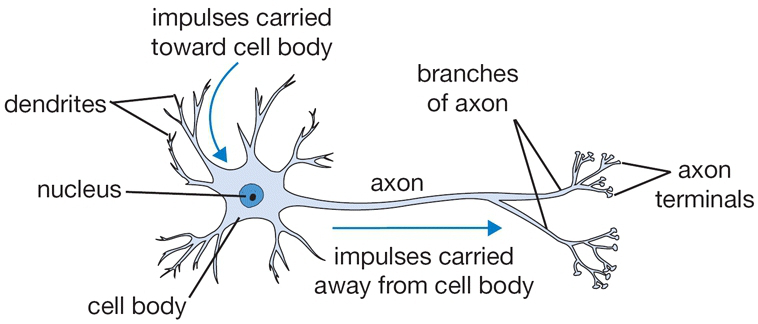
\includegraphics[width=1\textwidth]{fig/neuron}
            \caption{Biological neuron\cite{cs231n_part1}}
            \label{fig1}
    \end{minipage}
    \begin{minipage}{0.4\textwidth}
        \centering
            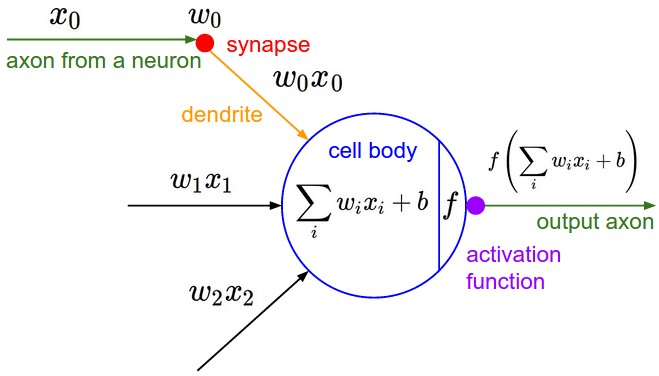
\includegraphics[width=1\textwidth]{fig/neuron_model}
            \caption{Mathematical model of a neuron\cite{cs231n_part1}}
            \label{fig2}
    \end{minipage}
\end{figure}

\noindent To simulate these signals, an ANN uses a mathematical model as illustrated in \textbf{Fig. \ref{fig2}}, where the signal is multiplied by the weight of a connection. The weight of a specific connection controls how much the unit on one end influences the unit on the other end. The sum of all input signals are computed at the cell body of the unit, and a constant, \textit{b}, is added from a bias unit. A bias unit is another unit that influences the output without interacting with the actual data. The unit fires an output signal determined by its activation function by performing a specific mathematical operation on the result.

\subsection{The Multi-Layer Perceptron}

\noindent The simplest form of an ANN is the single layer perceptron, which consists of only one layer of output nodes. This network can only learn linearly separable patterns. To allow the learning of complex patterns, more layers need to be added, resulting in the multi-layer perceptron (MLP). As layers are added, the depth of the network increases. This is the reason why the use of MLPs is referred to as "deep learning".\\

\noindent There are several different classes and types of ANNs. We will focus on the standard feed-forward neural network, and thus we will use the term ANN when referring to such a network. In a feed-forward network, all connections are directed from one layer to the next layer, and there are no cycles or connections between units in the same layer. \\

\noindent The first layer of an ANN is called the input layer. Similarly, the last layer is called the output layer. All layers in between are referred to as hidden layers, and are usually fully connected layers. This means that each layer node is connected to every node in the preceding layer. A layer can also be a convolutional layer or a pooling layer, but these cases will be covered later, in section 2.2.

\subsection{Activation Functions}

\noindent The common behaviour of all activation functions is that they define the output of a unit given a set of inputs. There are a great variety of activation functions in use, but we will only describe those most commonly used and thus considered in our implementation. The mathematical function of three of these are plotted in \textbf{Fig. \ref{activationfuncs}}. \\
\begin{figure}[H]
    \begin{minipage}{0.3\textwidth}
        \begin{tikzpicture}
            \begin{axis}[
                title = {Sigmoid function},
                axis lines = center,
                xtick={-10, -5, 5, 10},
                ytick={0, 0.2, 0.4, 0.6, 0.8, 1.0},
            ]
            \addplot [
                domain=-10:10,
                samples=100,
                color=blue,
            ]
            {1 / (1 + e^-x)};
            \end{axis}
        \end{tikzpicture}
    \end{minipage}
    \begin{minipage}{0.3\textwidth}
        \begin{tikzpicture}
            \begin{axis}[
                title = {Tanh function},
                axis lines = center,
                xtick={-10, -5, 5, 10},
                ytick={-1.0, -0.5, 0, 0.5, 1.0},
            ]
            \addplot [
                domain=-10:10,
                samples=100,
                color=blue,
            ]
            {(2 * (1 / (1 + e^-(2*x)))) - 1};
            \end{axis}
        \end{tikzpicture}
    \end{minipage}
    \begin{minipage}{0.3\textwidth}
        \begin{tikzpicture}
            \begin{axis}[
                title = {ReLU function},
                axis lines = center,
                xtick={-10, -5, 5, 10},
                ytick={2, 4, 6, 8, 1.0},
            ]
            \addplot [
                domain=-10:10,
                samples=100,
                color=blue,
            ]
            {max(0, x)};
            \end{axis}
        \end{tikzpicture}
    \end{minipage}
    \caption{The most commonly used activation functions}
    \label{activationfuncs}
\end{figure}

\subsubsection{Sigmoid}

The sigmoid activation function is mathematically defined as $\sigma(x) = 1/(1 + e^{-x})$. The function takes a number as input, and outputs a number within a continuous range from 0 to 1. It is commonly used as the activation function for the output node of a binary classification problem. Apart from this, the other activations functions tend to be preferred to the sigmoid function because of its drawbacks. The first drawback is that the outputs are not centered around zero, which can cause the network to display undesirable behaviour. A bigger drawback is that the activation saturates, meaning that the units output mostly 0 and 1 instead of anything in between, and thus the gradient at these regions is very low. If the gradient falls to zero, the network will stop learning.

\subsubsection{Softmax}

The softmax activation function is a variant of the sigmoid function. Instead of being used in binary classification, it is used for the output nodes of a multiclass classification problem, where the goal is to classify instances into one of more than two classes. The mathematical equation for the softmax function is $f(x) = e^x/\sum_{j=0}^k e^{x_j}$. It calculates the probability distribution of each target class over all possible target classes. A convenient result of this is that the sum of all probabilities will be equal to one. Note that the softmax function is not used in middle nodes, but only as the activation function of output nodes.

\subsubsection{Tanh}

The tanh activation function is a scaled version of the sigmoid function. Its mathematical function is $tanh(x) = 2\sigma(2x) - 1$. The scaling causes the tanh function to output numbers within the range of -1 and 1. This makes the output zero-centered, thus avoiding the first drawback of the sigmoid function. Even though the tanh function still suffers from saturation, it is preferred to the sigmoid function.

\subsubsection{ReLU}

The Rectified Linear Unit (ReLU) activation has the mathematical function $f(x) = max(0,x)$. This means that it is very close to linear; thresholding the input at zero, but keeping any value above. It has become highly popular, and is in general the activation function of choice. It is non-saturating, and has been found to speed up the convergence of the learning. The computation of the function is also inexpensive compared to the sigmoid and tanh functions. The only problem with the ReLU function is the possibility of "dead" units, i.e. units that will never activate. Generally, adjusting the learning parameters can prevent this, but there have also been several attempts to fix this issue, for instance using so called PReLU or Maxout units.

\subsection{Training a Network} \label{training-sec}

The weights of a model can be learned by training the model on a set of input and output values, a task which is called supervised learning. The weights are usually initialized to small, randomly generated numbers. The learning process runs for a number of epochs, i.e. the number of times the learning algorithm will see the entire training set. Often, the data is split into so called batches when passed to the algorithm. The number of training examples in a batch is referred to as the batch size.

\subsubsection{Data Preprocessing} % usikker på hvor denne hører til

A common form of data preprocessing that we will employ is mean subtraction. This involves zero-centering the data by subtracting the mean across each of its individual feature, to ensure that the features are in a similar range. For images, this would be the values of the R, G and B channels. Note that the mean should only be computed for the training data, but it still has to be applied to the test data.

\subsubsection{Overfitting and Dropout}

The training data of an ANN might often be noisy and incomplete. Overfitting is when the ANN learns the details and noise of the data too well, so that it impacts the performance of the ANN on new data in a negative manner. An effective and simple regularization technique to prevent overfitting is dropout, where randomly selected units are ignored during training. A node is dropped out with a given probability each weight update cycle. This makes the network less sensitive to the specific weights of the units, and results in a more generalized network that is less likely to overfit to the training data.

% this section probably still needs a lot of fixing

% X skrive om zero-centered data, mean-centered osv
% X nevne weight initialization
% X overfitting --> dropout
% hyperparameters ??? mentions learning rate in gradient descent, and briefly describes it

\subsubsection{Loss Function}

\noindent The goal of an ANN is to find a function that solves a certain problem, or more specifically, finds an optimal solution to the problem. The definition of this optimal solution is that given a loss function, there are no other solution with a lower loss value. The loss function is in that sense a measure of how far away a solution is from an optimal solution. The goal of the learning process is thus to find a function with the smallest possible loss. There are several loss functions that can be used in an ANN, suited for different purposes. For classification tasks where you want to minimize the number of misclassified training pairs, cross-entropy is the natural choice.

%  Cross entropy cost is appropriate to classification where the goal is to minimize the number of mis-classified training samples by imposing an exponentially increasing error the closer an output comes to being "1" when it should be "0", and vice versa.

\subsection{Gradient Descent and Backpropagation}

\noindent To optimize the loss, we can use an algorithm called gradient descent, which minimizes any function iteratively. The algorithm makes the learning process a repeated loop of evaluating the gradient, and then updating the weights based on this gradient. The simplest form of this algorithm, also called the vanilla version, is shown in \textbf{Code \ref{code:1}}. \\

\begin{listing}[h!]
\begin{minted}
[
frame=lines,
framesep=2mm,
baselinestretch=1.2,
fontsize=\footnotesize,
linenos
]
{python}
for i in range(epochs):
    weights_grad = evaluate_gradient(loss_function, data, weights)
    weights += - learning rate * weights_grad
\end{minted}
\caption{Vanilla gradient descent}
\label{code:1}
\end{listing}

\noindent First, the algorithm evaluates the gradient of the loss function for the whole training data set with respect to the current weights. This is done using an algorithm called backpropagation. Often, the term is used to refer to the complete process of repeatedly computing the gradient and updating the weights. Each iteration of computing the gradient involves two steps: forward propagation and backward propagation, also known as forward pass and backward pass, respectively. The forward propagation is simply the propagation of an input through the network in order to generate an output. In the backward propagation step, the loss between the generated output and the desired output is computed, and the error is propagated backwards to the previous layers. The error values are then used to calculate the gradient. The next step of gradient descent is to adjust the weights, based on the evaluated gradient and a chosen learning rate. The learning rate controls the magnitude of the update, and is a crucial network hyperparameter. This process is repeated for a pre defined number of epochs.

\subsubsection{Stochastic Gradient Descent}

The vanilla version of gradient descent is also called batch gradient descent. A batch of data is a portion of the training data, in this case the entire training data set. The gradient is computed over such a batch, which is slow and expensive in terms of memory. There are a number of different ways to optimize gradient descent by extending the vanilla version. Stochastic gradient descent (SGD) represent one of these optimizations. In this case, the gradient is computed over mini-batches consisting of only one training pair. This is a special case of the more general mini-batch gradient descent, which computes the gradient over batches of the training data, instead of the entire set. SGD refers to both mini-batch gradient descent, as well as the special case of stochastic gradient descent. Usually, it is more efficient to compute the gradient over a number of training pairs instead of just one. Even though SGD is much more efficient than the vanilla version, it also has its drawbacks. Therefore, a number of improved algorithms have been developed.

\subsubsection{Adding Momentum}

One way to improve SGD is to add momentum. SGD can get stuck in local optima, and adding momentum can help it accelerate in the right direction. A further improvement is the Nesterov momentum, which adds some notion of where SGD is heading by approximating the next position.

\subsubsection{Adaptive Learning Rate Methods}

Adaptive learning rate methods are algorithms that automatically adapts the learning rate to the parameters. They are all quite similar, and perform thereafter. In general, SGD often finds a minimum, but these methods can help to achieve convergence faster, and requires no tuning of the learning rate. The algorithms are usually implemented with a decent default starting value. Adagrad was the first adaptive learning rate method proposed, and the later additions are extensions of it. Its weakness is that the learning rate decreases and eventually becomes close to zero. AdaDelta and RMSprop are methods that try to overcome this flaw, and they are close to identical. Another option, Adam, adds some form of momentum to the optimization, and therefore might be the best overall choice.

\section{Convolutional Neural Networks}

A variation of the traditional ANN, convolutional neural networks (CNNs) are especially well suited for handling input data that can be arranged in a grid-like topology. These types of networks are commonly used in situations where the processing of images is required, but can be applied to input of any dimension. We will, however, concentrate on the convolution of images, as it is of most relevance to the thesis. \\

\noindent A typical CNN architecture involves multiple convolutional layers as the main body of the network, interspersed with pooling layers, before ending with one or more fully connected layers. A convolutional layer employs a mathematical operation called convolution, from which the name of both the layer and the network type is derived. Before explaining the convolutional layer and the pooling layer, as well as a convolutional layer variant called the transposed convolutional layer, we review the convolution operation and its matrix multiplication counterpart.

\subsection{Convolution Operation}

Generally, convolution can be defined as an operation on two functions, $x$ and $w$, of a real-valued argument, $t$:

\[ s(t) = \int x(a)w(t-a) da \]

\noindent The operation is typically denoted $s(t) = (x*w)(t)$. While the above definition is for arguments in the continuous range, data in computer applications is usually discrete. If we assume that $x$ and $w$ are only defined on discrete values of $t$, the convolution operation can be discretized:

\[ s(t) = (x*w)(t) = \sum_{a=-\infty}^{\infty} x(a)w(t-a) \]

\noindent In CNN terminology, $x$ and $w$ represents the input the convolution kernel, respectively. For a network, the input and kernel are usually multidimensional arrays, the first containing data and the second containing the network parameters, or weights. Because these arrays are finite, we can assume that the functions are zero for elements that reside outside the arrays' range. The infinite summation in the discrete convolution operation can then be reduced to a summation over a finite number of array elements. In addition, it is often desirable to perform convolutions over multiple axes at a time. The convolution operation for a 2D image input $I$, using a 2D kernel $K$, would then be defined:

\[ S(i, j) = (I*K)(i, j) = \sum_{m} \sum_{n} I(m, n) K(i-m, j-n) \]

\noindent Since convolution is commutative, the following is equivalent:

\[ S(i, j) = (K*I)(i, j) = \sum_{m} \sum_{n} I(i-m, j-n) K(m, n) \]

\noindent The commutative property is a result of the kernel being flipped relative to the input, such that the input index increases with $m$, while the kernel index decreases. This property is not essential in practice and many ANN libraries implement cross-correlation instead, calling it convolution. In reality, cross-correlation is equivalent to convolution without the kernel flipping:

\[ S(i, j) = (I*K)(i, j) = \sum_{m} \sum_{n} I(i+m, j+n) K(m, n) \]

\noindent An example of an application of cross-correlation on 2D input can be seen in Fig. X Following convention, we will not differentiate between the two approaches any further and refer to both as convolution operations. 
 
\subsection{Convolution as Matrix Multiplication} \label{conv-matrix}
 
Discrete convolution can be represented by a matrix multiplication and there are multiple ways to define the operation. The definition presented here was chosen as it allows the differences between convolution and transposed convolution to be easily demonstrated in section X. \\

\noindent Consider a discrete convolution of a 4x4 input matrix with a 3x3 kernel matrix. To perform this convolution via matrix multiplication, we must first unroll the input matrix from left to right and top to bottom, reshaping the input into a 16-dimensional vector $I$. The kernel must also be modified, creating a sparse matrix $K$, where $w_{ij}$ is the element at row $i$ and column $j$ in the original kernel:

\[
    K = 
    \left(
    \begin{smallmatrix}
    \textit{$w_{00}$} & \textit{$w_{01}$} & \textit{$w_{02}$} & 0 & \textit{$w_{10}$} & \textit{$w_{11}$} & \textit{$w_{12}$} & 0 & \textit{$w_{20}$} & \textit{$w_{21}$} & \textit{$w_{22}$} & 0 & 0 & 0 & 0 & 0 \\
    0 & \textit{$w_{00}$} & \textit{$w_{01}$} & \textit{$w_{02}$} & 0 & \textit{$w_{10}$} & \textit{$w_{11}$} & \textit{$w_{12}$} & 0 & \textit{$w_{20}$} & \textit{$w_{21}$} & \textit{$w_{22}$} & 0 & 0 & 0 & 0 \\
    0 & 0 & 0 & 0 & \textit{$w_{00}$} & \textit{$w_{01}$} & \textit{$w_{02}$} & 0 & \textit{$w_{10}$} & \textit{$w_{11}$} & \textit{$w_{12}$} & 0 & \textit{$w_{20}$} & \textit{$w_{21}$} & \textit{$w_{22}$} & 0 \\
    0 & 0 & 0 & 0 & 0 & \textit{$w_{00}$} & \textit{$w_{01}$} & \textit{$w_{02}$} & 0 & \textit{$w_{10}$} & \textit{$w_{11}$} & \textit{$w_{12}$} & 0 & \textit{$w_{20}$} & \textit{$w_{21}$} & \textit{$w_{22}$} \\
    \end{smallmatrix}
    \right)
\]

\noindent Executing the matrix multiplication $KI$ would then produce a 4-dimensional vector, which could be reshaped into the 2x2 matrix we expect from the convolution. Thus, the matrix multiplication is equivalent to the regular convolution operation.

\subsection{Convolutional Layer}

To reiterate, a convolutional layer employs convolution to compute its output, unlike traditional fully connected layers. As a result, convolutional layers incorporates certain advantageous concepts, namely sparse connectivity, parameter sharing and equivariance to translation.

\subsubsection{Sparse Connectivity}

As implied by the name, every unit in a fully connected layer is connected to every unit in the previous layer. In convolutional layers, however, the convolution kernel is typically smaller than the input, causing sparse connectivity. Each unit in the layer is then only connected to a subset of the units in the previous layers, as dictated by the kernel. Consequently, the output of each unit can be computed using fewer mathematical operations. Sparse connectivity also results in a lower amount of weights compared to a fully connected layer, and even drastically so when combined with the effects of parameter sharing.

\subsubsection{Parameter Sharing}

Where each weight of a fully connected layer is only used once, each weight in a convolutional layer is used multiple times. When convolving, the kernel is applied at several different areas of the input, reusing the parameters of the kernel across the input. Every unit in the convolutional layer then uses the same kernel weights as the other units to connect to the layer below. In this situation, the weight are said to be shared among the units. Additionally, the parameter sharing characteristic means that the kernel parameters learned in training are location independent.

\subsubsection{Equivariance to Translation}

The equivariance property of convolutional layers are caused by the particular form of parameter sharing. Specifically, convolutional layers have equivariance to translation, which means that if the input of the layer experiences any translation changes, then the output changes in the same way. Consider a convolution with an image input, where the kernel parameter values are set to detect the edges of an object. The convolutional layer would then create a map of where the edges are located. Because of the equivariance property, if the object shifts to another location in the image, the edge mapping would shift accordingly.

\subsubsection{Convolution for Feature Detection}

Together, the discussed concepts make convolutional layers a powerful addition to the ANN toolbox, especially for image input. As mentioned, the kernel parameters can be chosen so the convolutional layer detects edges. Since the same parameters are used across the input, the layer will be able to discover edges at any location in the image. Edges might not be the only thing of interest, and using a kernel with different parameters could provide a mapping of another feature, for example a corner. Consequently, convolutional layers often employ multiple different kernels, which differ in parameter values, but are equal in size. In truth, detecting edges with a single kernel would only allow the layer to identify edges of a specific orientation, for example horizontal of vertical. With several kernels, the layer can detect edges of any orientation, as well as many other simple features. \\

\noindent A second convolutional layer could be added, convolving the output of the previous layer with its own specialized kernels. This enables the detection of features that are composed of the features found in the preceding layer. With additional layers, the features can become even more complex, each building on the ones below. Stacking convolutional layers make CNNs able to perform remarkably well on image input, for example in face recognition. Then, lower layer kernels start by detecting simple features, like edges, which later kernels can use to detect more complex patterns, like eyes or mouths. Layers even deeper in the network can then use that output to identify complex structures like faces. While the sparse connectivity between layers might be thought to hinder such complexity, the connectivity of units in later layers take on a pyramid-shaped pattern, as throughout the layers they become indirectly connected to a increasingly larger portion of the units below and, ultimately, the input. Because of the feature detecting abilities of convolutional layers, their kernels and outputs are often referred to as filters and feature maps, respectively. \\

\noindent When convolving with several kernels, the output of a convolutional network gains a new dimension. On a 2D image, a 2D kernel will produce a 2D output. With several kernels, the output assumes a 3D shape, with the kernel number following the depth axis. In reality, the image input is also usually 3-dimensional, on account of the color axis for RGB images. Thus, convolutional layers often operate with 3D input, either the original image or the feature map of the layer below. In these situations, kernels are also 3-dimensional, with sparse connectivity in the spatial dimensions, but full along the channel (color/kernel) axis. Used on feature maps, these kernels can then consider all the different features identified simultaneously, enabling the complex feature detection. The output will be 3-dimensional, as before. If the next layer is fully connected, it is common to flatten the output. 

\subsection{Hyperparameters in a Convolutional Layer}

The effects of the hyperparameters described here are mostly structural and affects the single convolutional layer for which they are used. In a CNN, however, the hyperparameters of one layer can have widespread consequences, which depend upon the domain and network architecture. Instead of an exhaustive explanation of the potential ramifications, we present the concepts and more immediate effects. There are five important hyperparameters to consider: the activation function, amount of filters, filter size, strides, and padding. 

\subsubsection{Activation Function}

The activation function in a convolutional layer is employed similarly as in a fully connected one, computing the output of every unit in the layer. It is typically chosen to be a ReLU function, to add non-linearity to the network and ensure strictly positive feature maps. The latter is useful as a negative activation for feature detection is not meaningful.

\subsubsection{Filter Amount and Size}

Not suprisingly, the filter amount denotes how many different filters the layer should use and the filter size determines the spatial size of the filters, which is usually small, e.g. 3x3. As previously mentioned, a convolutional layer can use multiple filters to search for different features. Intuitively, the amount of filters a layer uses dictates how many different features it can extract. In addition, it also decides the depth of the layer output. The filter size affects the output size as well, which is explained in more detail when reviewing padding.

\subsubsection{Strides}

The stride refers to the distance between filter applications in units. For image input, it applies in both spatial directions, meaning two separate strides must be specified. In a basic convolution, with single strides and no padding, the filter would be applied to every unique (spatial) neighborhood of units that matches the filter size. For a 4x3 input and a 2x2 filter, there exist six such neighborhoods, as implied by Fig. X. Each filter region is then a single step away from any another, both vertically and horizontally. If we increase horizontal stride to two, the filter will only be applied to every second neighborhood in that direction. As a result, four regions of the input would be convolved, creating a 2x2 feature map. By increasing both strides to two, the feature map would be further reduced to 2x1, as there would not be enough units for two filter regions that were two steps apart in the vertical direction. The strides can be further increased, but they are rarely set to large values. The purpose of the strides is to downsample the input, reducing computational cost at the expense of finer feature extraction. Although increasing the filter size would also diminish the feature map, it would limit the layer's feature detection capabilities, making larger strides the preferred approach.

\subsubsection{Padding}

Padding has the opposite effect of strides and is used to either retain the spatial size of the input or increase it. Even without strides, any input passed through a convolutional layer will decrease in height and width by one less than the filter height and width, respectively. This happens because the layer will only apply convolution where the filter fits and not at the border of the input, where parts of the filter fall outside. If the layers keeps diminishing the input, it puts a restriction on the amount convolutional layers a network can employ before the output becomes too small for any meaningful use. An alternative is to use smaller filters to reduce shrinkage, but this limits the expressive power of the network similar to the layer restriction. However, by zero padding the input before applying filters to it, the problem can be avoided. When padding is involved, convolution can be separated into three categories: valid, same and full. Valid convolution occurs in the aforementiond case, with no padding, where convolution is only applied at regions that fully contain the filter. In same convolution, padding is added to the layer input to make the layer output have the same spatial size as the unpadded input. However, the units at the border of the input will still be involved in less convolutions and therefore influence less layer units. This is taken into account in full convolution. Here, padding is added so that every input unit is involved in an equal amount of convolutions. Some layer units will then be a function of fewer input units, which can interfere with the learning of decent filters. Consequently, valid or same convolution is usually preferred over the full variant.

\subsection{Training a Convolutional Layer}

Training a convolutional layer is similar to training a fully connected one, as explained in section \ref{training-sec}. As discussed in section \ref{conv-matrix}, convolution can be thought of as a matrix multiplication. Following the example from that section, we use the kernel matrix K to define the backward pass for convolutional layers. While we have established that convolutional layers often handle input, output and kernels with three dimensions, we use 2D matrices here to simply illustrate the backward pass approach. To that effect, we also assume single strides and no padding. 

\subsubsection{The Backward Pass}

The forward pass has already been established to be the matrix multiplication $KI$, using the 16-dimensional input vector I, which produces a 4-dimensional output vector. To do a backward pass, the transposed version of $K$, $K^T$, would be used. This transposed version of the convolution matrix allows the backward pass to receive a 4-dimensional vector as input and produce a 16-dimensional vector as output, which can be reshaped to the original 4x4 size. If the error is being backpropagated, the backward pass would use a loss vector, L, to compute $K^T L$. 

\subsubsection{Connectivity Pattern Conservation}

In a forward pass, a single entry in the output vector is only affected by a subset of the entries in the input vector and always the same ones. The backward pass has the same connectivity pattern between the entries in the input and output vector, only in the reverse order. These connectivity patterns are compatible since both passes are defined by $K$. In context of the example, the first entry (index 0) of the forward pass output vector would be connected to the input vector entries with index 0-2, 4-6, and 8-10, as implied by the first row of $K$. Subsequently, the backward pass output vector entries with index 0-2, 4-6, and 8-10 would be connected to the first entry in the input vector, as implied by the first column of $K^T$. The conservation of this pattern affirms the validity of the backward pass approach.

\subsubsection{Effects of Strides and Padding}

Strides and padding have an effect on the output size of a layer, as previously explained. These two, in combination with input size and filter size, determine the spatial size of the feature maps. Using different stride and padding policies, forward passes for multiple inputs of varying size can produce feature maps of similar size. As a result, performing a backward pass transposed convolution will not necessarily be as straightforward as in the basic case, with single strides and no padding. The details on how transposed convolution can be performed with the various combinations of strides and padding is not of great importance to the thesis and will be described no further. It suffices to be aware of issue, which explain why some implementations require the desired output size to perform transposed convolution.

\subsection{Transposed Convolutional Layer}

A transposed convolutional layer (also known as a fractionally strided convolutional layer) is almost identical to a regular convolutional layer, with an important distinction: the forward and backward passes are swapped compared to a convolutional layer. Where a regular layer uses $K$ and $K^T$ for the forward and backward pass, respectively, the transposed convolutional layer would use $K^T$ and $K$ for the forward and backward pass, respectively. As $(K^T)^T=K$, the transposed convolutional layer is simply a regular convolutional layer using transposed convolution matrices, hence the name. Because both the passes are defined by $K$, the connectivity pattern found in regular layers also holds for transposed convolutional layers. \\

\noindent Transposed convolutional layers can be implemented with the same hyperparameters as regular convolutional layers. In this case, the strides and the padding specified usually applies to the convolution operation in the backward pass, which then dictates how the transposed convolution in the forward pass will behave. These layers are typically found in networks used to reconstruct some input from the output of another CNN. An example is deconvolutional neural networks (DCNNs), which try to reconstruct an input image, with certain features highlighted, from a set of feature maps. DCNNs will be explored further in the section of this chapter covering visualization techniques.

\subsection{Pooling Layer}

Pooling layers are a common occurrence in CNNs and they can employ multiple types of pooling functions. A pooling function is applied to various regions of the input and outputs a summary statistic of the units for each region. Popular ones include max pooling, average pooling, and weighted average based on distance from pooling center. Of these, only max pooling is relevant for the thesis and will be described in this section. \\

\noindent Max pooling layers are fairly straightforward. Given an input, a layer determines several pooling regions and outputs the maximum value for each region. Pooling regions are similar to convolutional filter regions, with the exception that they are usually singular in depth. The region spatial size is decided by a pooling size hyperparameter. Pooling is also typically restricted to full regions, e.g. a 3x3 pooling will not be applied to a 3x2 region at the border of the input. Like convolutional layers, however, pooling layers can employ strides and padding to influence how input is processed.

\subsubsection{Translation Invariance}

The benefit of pooling layers is that they make a network approximately invariant to small translations of the input. Remember that convolutional layers have equivariance to translations, so their output shifts similar to the input. In pooling layers, a small shift of the input will only affect the output of the regions that gain a new maximum value. This only happens in regions where the previous max unit is shifted out or if a unit with greater value is shifted in. In practice, most of the output will remain unchanged, providing approximate invariance. It is a useful property to have if it is important to detect whether a feature is present, but its exact location is less significant. Some times, the location of a feature is important, for example if we are looking for a corner defined by the connection of two edges, the edge locations must be preserved properly to examine whether they join or not.

\subsubsection{Training}

CNNs with max pooling layers can still be trained with gradient descent and backpropagation. There does not exist an inverse to the max pooling function to use in a backward pass, but that problem can be solved using so called switches, which are routings between input and output units. In a forward pass, simply save which input units had a maximum value and which output unit they correspond to. These routings can then be used in backpropagation to pass the gradient back to the right unit. 


\section{Visualization}

When using ANNs to solve complex problems the inner workings can be difficult to understand. It is not unlikely that the network is highly non-linear and requires millions of parameter values to obtain a desirable performance level. In these cases, it is hard to gain insight about the network's performance by examining the parameter values directly, both because of the unfeasible amount of values and each value's relative insignificance by itself. However, when applying ANNs to tasks in the image domain, there are several ways to help us understand the inner workings of the network by presenting information in the same readable format as the input. Aside from the fact that images more suited than numbers for human readability, there exists several techniques that utilizes the connections in the network to produce visualizations. These images can then provide insight into a larger part of the network, spanning several layers, possibly the whole network. Through the use of these visualization techniques, the network can improved by making informed decisions, instead of employing a trial and error approach. 

\subsection{Training Progress Measurements}

Throughout training, the progress of the network is visualized in a simple line plot. Measurements are made of the standard network appraisal values, loss and accuracy, both on the training set data and, if provided, the validation set data. A typical thing to want to monitor, these values provide a means to explicitly evaluate a network's performance. Plotting the values against time, at certain batch intervals or at epoch completion, puts the current measurements in perspective, and makes the training progress, or lack thereof, easily discernible. The shape of the line plot could also be used to reveal undesirable values in the training hyperparameters. For example, if the learning rate is too large, the network is likely to vastly improve at first, only to have its progress quickly stagnate. In this case, both loss and accuracy plots would have distinct shapes that indicate a problem, without having to look at any of their actual values.

By including the validation values, one could also be able to identify the presence of overfitting, marked by a point where the validation accuracy begins to decline while training accuracy continues to rise.

\subsection{Layer Activations}

From yosinski paper, section 2: "Although this visualization is simple to implement, we find
it informative because all data flowing through the network can be visualized. There is nothing mysterious happening behind the scenes."

\textit{The activation output is most readable for the convolutional layers, and especially so for the earlier ones. The activations in convolutional layers can also be called feature maps, and the units in these maps typically share the same weight matrix, called the filter. The filter will, through backpropagation, learn to look for certain features, for example a horizontal edge. Applying the filter to the input creates the feature map, which can convey information about where the filter found the feature it was looking for. For deeper convolutional layers, these features become more complex and so does the input. It is the simplicity of their filters and input that make the earlier layers activations easier to interpret. Considering these filters, the activation output can be helpful to confirm that the network is progressing well, if the output is showing signs of activation in areas with similar features. These patterns should become more and more clear as training goes on, and when the activations start experiencing little or no change, the proper filters should be obtained.} \\

\noindent \textit{Additionally, in networks using ReLUs, a common activation function, the expectation of seeing sparse and localized activations can be confirmed, which is an indicator of the network learning properly. If some feature maps are entirely dark, with all pixel values zero, this can be a warning sign that the learning rate is too high. The particular filters are then rendered useless, and they have no possible way to recover \cite{cs231n_act}. }

\subsection{Saliency Maps}

\textit{A salience map is typically a black-and-white image with the same size as the input, where important pixels have a high value, and insignificant pixels have a low value \cite{salience}. Thus, the important regions can be easily identified by their brightness. A map for classification is specific to an image and a class, and it allows us to observe which parts of an image influences the network classification score the most. In other words, we can view which parts of an image that the network deems more important when deciding upon the classification score chosen. Such a map can be produced by efficiently using the back-propagation gradient of the output score with respect to the input image.} \\

\noindent \textit{In a face recognition case, the saliency would allow us to investigate what the network emphasizes, for example which facial regions are decisive in producing the identification output. We could also exploit salience maps for expression classification, creating maps to display which areas were the most influential for selecting the outputted expression results. By using the insight gained through salience maps, we would be able to confirm our beliefs that a network focuses on regions containing important feature information, and alert us to any peculiarities.}

\subsection{Deconvolution Network}

Modern networks that receive images as inputs are likely to have convolutional layers form the initial part of the network. This part is aimed at detecting certain features in the image, with the complexity of the features rising as the depth of the convolutional part increases. In such cases, we can utilize a visualization technique that employs a deconvolutional network, which can be thought of as a reverse convolutional network \cite{deconv_net}. The visualizations are used to interpret the feature activity in the intermediate layers of the original network. To obtain a visualization, an image is first fed to the original network to produce activations in its various layers. The activations of the convolutional part can then be processed and fed to the deconvolutional network to create a visualization of the pattern in the input image that was responsible for eliciting the given activations. This pattern can then reveal what a certain part of the original network finds important and what it is looking for in an image. \\

\noindent To build such a deconvolutional network, it is necessary to examine the original network we want to produce visualization for. Only the feature extracting part is of interest, and we can regard this part as a network on its own. The purpose of the deconvolutional network is to map the feature activity present in this convolutional network back to the input pixel space \cite{deconv_vis}. For a convolutional network consisting of convolution and max pooling layers, the corresponding deconvolutional network would consist of transposed convolution and unpooling layers in the opposite order of the original layers. In addition, where a ReLU activation function commonly follow each convolutional layer, they would precede transposed convolutional layers. In other words, a top-down examination the convolutional network would enable a bottom-up creation of the deconvolutional network. \\

\noindent The fact that a transposed convolution can reverse a convolution downsampling while maintaining a similar connectivity pattern makes them suitable for a deconvolutional network. A convolutional layer in the original network would apply their filters to the output of the previous layer (or the image input) and produce feature maps, which are then rectified by the ReLU activation function. In the deconvolutional network, the aim is to map the rectified feature maps back to convolution input, and this is where transposed convolution is used. By using the same filter weights in a transposed convolutional layer as in its corresponding convolutional layer, the deconvolutional network is able to create a mapping that is specific to the original network. \\

\noindent As previously mentioned, the input to the transposed convolution should first be passed through a ReLU activation function. In a convolutional layer, ReLU ensures that the feature maps outputted are strictly positive. For the convolution input reconstruction to be valid, the reconstructed feature maps used as input for the transposed convolutional layers must also be strictly positive. Passing the reconstructed feature maps through a ReLU activation function ensures this. \\

\noindent To reverse the effects of the max pooling layers of the original network, the deconvolutional network uses unpooling layers. Pooling, however, is not an invertible operation and the unpooling layers therefore focus on obtaining an approximation of the original max pooling input. The key to the approximation is to use a switch variable for each pooling region. When performing max pooling, these switches record the location of the chosen maximum in each region and pass the information to the unpooling layer. Here, they are used to place the entries in the unpooling input into the appropriate locations in the output. The result is an unpooling output that only has non-zero values in entries that correspond to the maximum entries in the pooling input. This reconstruction approach preserves the structure of how max pooling processes stimulus. \\

\noindent To utilize a constructed deconvolutional network, first the feature map output from a chosen layer in the original network must be produced. Before the feature maps are fed to the corresponding layer of the deconvolutional network, they must be processed. To visualize what a particular filter is looking for, all entries in the feature maps is set to zero, except the maximum entry in the filter's corresponding feature map. Only the maximum entry is left untouched to create a visualization that is able to convey what pattern in the input image activates that filter strongly. When the processed feature maps are inputted into the deconvolutional network, the layers will successively reconstruct the activity that was responsible for the chosen feature map activation until the input pixel space is reached. If visualizations for several filters are desired, the deconvolutional network has to run multiple times, each with feature maps only containing a single non-zero entry. \\

\noindent When the original network is applied to an input image, the switches created in its max pooling layers are specific for that image. The reconstruction from the processed feature maps are created using these switches and it will therefore resemble the input image. However, only the patterns that contribute towards the chosen feature map activation are reconstructed. The visualization outputted by the deconvolutional network will then be mostly blank, with a highlight of the important section of the image and its characteristics. Creating visualizations from several images for a single filter can reveal what the filter is looking for. For example, if a filter is trained to detect eyes, the reconstructions from this filter will repeatedly focus on image sections containing eye-like traits, as well as highlighting those traits. One could also have a single image and use several different filters to produce visualizations, which could reveal if the original network is capable exploiting the discriminative features in the image. If a network is supposed to locate faces, but none of the visualizations show any focus on the eyes, they could warn about flaws in the network and potentially explain poor performance. Conversely, if the visualizations cover a wide range of facial characteristics, they can provide reassurance about the quality of the network's feature utilization. \\

\noindent Visualizing for several layers can also shed light on the hierarchy of the filters, where the lower layers usually concentrates on low level features like edges and textures and the upper layers looks for more complex features, e.g. eyes. If a network experiences problems with upper layer filters, it is possible that these stem from poor filters further down. Applied during training, visualizations from different layers reveal when the filters of each layer converges. Typically, the lower layer filters converge quickly, while the upper layer filters develop at a much slower rate.


\subsection{Deep Visualization}

Whereas the previously discussed techniques (aside from plotting) are all dependent on a provided image to stimulate the network in order to create visualizations, deep visualization is not. Instead of examining the network's reaction to certain input, deep visualization aims to create images that represents what a selected part of the network is looking for. In order to achieve this, several steps are taken. \\

\noindent At first, an individual unit in the network must be chosen. It is this particular unit that the visualization will offer insight into. Secondly, an initial image should be created by setting every pixel to a random value. The dimensions should match the network's expected input. The next step is to compute an update to the image using gradient ascent. By iteratively updating the pixel values with the gradient of the image with respect to the loss of the chosen unit, the technique is able to produce images that maximally activate the unit. The idea is that images that cause strong activation in the unit would resemble the object or type of input that the unit looks for, i.e. its learned features. However, images produced from gradient ascent alone are inclined to contain certain "hacks" to influence the activation. These hacks, like extreme pixel values and structured high frequency patterns, guide the process away from natural, interpretable images. Fortunately, this behaviour can be suppressed. By employing regularization techniques to deter the evolution of hacks in the image, deep visualization is able to produce visualizations that are able to reveal the learned features of the unit. By repeating these two steps, updating the image with the gradient and then regularizing it, the process will eventually result in a viable visualization. When updating the image with the gradient, there can also be a learning rate attached, to accelerate (or decelerate) learning. It is worth noting that the process is stochastic as a result of the the random initial images. Producing several visualizations for a single unit would therefore display certain variances. These variances in turn reveal the invariances learned by the unit. \\

\noindent As an example, consider a network trained on classifying certain objects from images. In its last layer, this network has a unit which activates to classify the object in the input image as a cat. If this unit is selected for deep visualization, the resulting images should display various catlike features, e.g. four legs, tail, furry texture, particularly shaped faces, etc. If the output unit visualizations contain the expected features, confidence in the network is reinforced. However, if the features portrayed are irrational or intangible, it signals potential issues with the network. Assuming the network is able to classify a cat, it most likely contains parts that look for eyes as well. As deep visualization can produce images for any units in any layer, a hidden unit which activates on eyes could also be visualized. In that case, eyelike features should gradually become discernable in the once random image. Visualizing for a wide selection of hidden units can be helpful to understand the scope of the network's feature learning abilities. Ultimately, deep visualization can aid in understanding the network and whether it is looking for sensible features. \\

\noindent Regularization is the key to producing interpretable visualizations and the techniques used are $L_2$ decay, Gaussian blur and clipping based on specific attributes. While each is somewhat beneficial alone, they are even more effective when used in an ensemble. Before examining some suggested hyperparameters for the various regularization techniques, each technique is explained more thoroughly.

\subsubsection{$L_2$ Decay}

Employing $L_2$ decay is a common regularization technique for ANNs, where it is used to penalize large weight values. In these cases, the weights are linearly decayed towards zero with a chosen regularization strength. In deep visualization, $L_2$ decay is similarly applied to the visualization, where it is used to penalize extreme pixel values and prevents them from dominating the image. This is desirable as extreme pixel values are neither naturally prevalent nor useful for visualizations.

\subsubsection{Gaussian Blur}

Without regularization, an image generated from deep visualization has a tendency to contain a great deal of high frequency information, i.e. the pixel values are often radically different from that of their neighbours. While natural images do contain some high frequency information, for example at edges of objects, an excessive amount of it leads to unrealistic and uninterpretable visualizations. To combat this problem, Gaussian blur is applied as a regularization technique. The blurring makes transitions between pixels smoother, lowering the amount of high frequency information. \\

\noindent Of the techniques implemented, Gaussian blurring is the most computationally expensive. To reduce the cost, blurring can be performed only at certain intervals, using a blur kernel with a greater width. A single application of blurring with a large width kernel is equivalent to blurring multiple times with a small width kernel. Although the image will change slightly in between applications, the desired effect will be similar. 

\subsubsection{Clipping Based on Value, Norm and Contribution}

Another characteristic of images produced using deep visualization is an abundance of non-zero pixel values. In general, natural images contains a myriad of information aside from the primary focus. While not necessarily essential to the network, the secondary information will influence it nonetheless. In the visualizations, it manifests as disruptive non-zero pixel values. A subset of pixels will show the main object or type of input that excite the chosen unit and these are the focal point of the visualization technique. The other pixels, however, will still generally influence the gradient, each with a minor contribution to raise the activation. As a result, unwanted patterns will emerge in the visualization, disturbing the primary focus and cluttering the image. To prevent this behaviour, these disruptive pixels should be set to zero, which can be handled by using clipping regularization based on different attributes, namely value, norm and contribution. \\

\noindent Clipping based on value is rather straightforward. If the absolute value of a pixel in the visualization is below a set threshold, set the pixel value to zero. For an RGB-image, each color value can be examined separately. Although using values for clipping is not very complicated, it is neither very sophisticated. Another approach is to clip pixels based on their norm. The norm of each pixel would be computed over their color channels, and each pixel with a norm under the chosen limit would be set to zero. Finally, the pixel contributions to the unit activation can be used. The pixel contributions could be found by measuring how activation changes when each pixel is set to zero, but it would require a forward pass for every pixel and therefore be excessively expensive. Instead, the pixel contributions can be approximated by the elementwise product of the visualization and the gradient. For an RGB-image, each pixel contribution would be the sum of its color channel contributions. Normally, a pixel would be clipped, i.e. set to zero, if the absolute value of its contribution is below a set threshold. This would discard pixels which have a small contribution in either a positive or negative direction. Alternatively, one could use the contributions without computing their absolute values. In this case, pixels which greatly affect the activation in a negative manner are more likely to fall beneath the threshold and be clipped. The arguments against this is that the approximation made limits the validity of such large shifts and that the gradient ascent will handle these pixels iteratively. Thus, it could prove better to restrict regularization to only clip pixels that are considered to have an insignificant contribution value. 

\subsubsection{Regularization Hyperparameter Values}

Through a random hyperparameter search, \cite{deepvis} found several useful combinations that create visualizations with certain desirable characteristics. Not all of the previously described regularization techniques are included, however. Both clipping based on value and clipping based on contribution are included in \cite{deepvis_web}, but not in \cite{deepvis} (the latter is briefly mentioned). As a result, they are not included in the hyperparameter suggestions, but have been explained for the sake of diversity. \\

\noindent Denoting $L_2$ decay rate as $\theta_{decay}$, blur kernel width as $\theta_{b\_kernel}$, blur interval as $\theta_{b\_interval}$, norm percentile threshold as $\theta_{norm}$ and absolute contribution percentile threshold as $\theta_{abs\_contr}$, the hyperparameter combinations are:

\begin{table}[!h]
\begin{center}
\begin{tabular}{|c|c|c|c|c|}
\hline
\textbf{$\theta_{decay}$} & \textbf{$\theta_{b\_kernel}$} & \textbf{$\theta_{b\_interval}$} & \textbf{$\theta_{norm}$} & \textbf{$\theta_{abs\_contr}$} \\ \hline
0 & 0.5 & 4 & 50 & 0 \\ \hline
0.3 & 0 & 0 & 20 & 0 \\ \hline
0.0001 & 1.0 & 4 & 0 & 0 \\ \hline
0 & 0.5 & 4 & 0 & 90 \\ \hline
\end{tabular}
\end{center}
\caption{Hyperparameters found in random search, with useful combinations located in rows}
\label{tab:reg_hyperparams}
\end{table}

\noindent The four combinations produce visualizations that complement each other. The first one (at the first row) can be used to produce images that show a sparse set of important regions. The second tends to result in images with high frequency patterns. The third favors images with low frequency patterns. Finally, the fourth one generates visualizations with dense pixel data. Used separately, the most beneficial images can be developed from the third combination, although more insight can be gained by examining visualizations from all four combinations at once.


\section{Transfer Learning}

\section{Face Recognition}

\textit{Can probably use a lot from the specialization project here.}

\section{Facial Expression}

\textit{Here as well.}

\cleardoublepage